\documentclass{article}

\usepackage{graphicx}
\usepackage{rotating}
\usepackage{amsmath}
\usepackage{fancyhdr}
\usepackage{listings}
\usepackage{xcolor}
\usepackage{color}
\usepackage{textcomp}
\usepackage{float}
\usepackage{multirow}
\usepackage[sorting=none]{biblatex}
\usepackage[margin=1in]{geometry}
\usepackage[font={small,it}]{caption}
\usepackage{placeins}
\usepackage{xepersian}

%\DeclareMathOperator*{\btie}{\bowtie}
\addbibresource{bibliography.bib}
\settextfont[Scale=1.2]{B-NAZANIN.TTF}
\setlatintextfont[Scale=1]{Times New Roman}
\renewcommand{\baselinestretch}{1.5}
\pagestyle{fancy}
\fancyhf{}
\rhead{تکلیف ششم درس مبانی بینایی کامپیوتر}
\lhead{\thepage}
\rfoot{علیرضا ابره فروش}
\lfoot{9816603}
\renewcommand{\headrulewidth}{1pt}
\renewcommand{\footrulewidth}{1pt}
%%%%%%%%%%
\lstset
{
    language=[latex]tex,
    basicstyle=\ttfamily,
    commentstyle=\color{black},
    columns=fullflexible,
    keepspaces=true,
    upquote=true,
    showstringspaces=false,
    morestring=[s]\\\%,
    stringstyle=\color{black},
}
%%%%%%%%%%
%beginMatlab
\definecolor{mygreen}{RGB}{28,172,0} % color values Red, Green, Blue
\definecolor{mylilas}{RGB}{170,55,241}
%endMatlab
\begin{document}
%beginMatlab
\lstset{language=Matlab,%
    %basicstyle=\color{red},
    breaklines=true,%
    morekeywords={matlab2tikz},
    keywordstyle=\color{blue},%
    morekeywords=[2]{1}, keywordstyle=[2]{\color{black}},
    identifierstyle=\color{black},%
    stringstyle=\color{mylilas},
    commentstyle=\color{mygreen},%
    showstringspaces=false,%without this there will be a symbol in the places where there is a space
    numbers=left,%
    numberstyle={\tiny \color{black}},% size of the numbers
    numbersep=9pt, % this defines how far the numbers are from the text
    emph=[1]{for,end,break},emphstyle=[1]\color{red}, %some words to emphasise
    %emph=[2]{word1,word2}, emphstyle=[2]{style},    
}
%endMatlab
\begin{titlepage}
\begin{center}

\includegraphics[width=0.4\textwidth]{figures/IUT Logo.png}\\
        
\LARGE
\textbf{دانشگاه صنعتی اصفهان}\\
\textbf{دانشکده مهندسی برق و کامپیوتر}\\
        
\vfill
        
\huge
\textbf{عنوان: تکلیف چهارم درس ریزپردازنده}\\
        
\vfill
        
\LARGE
\textbf{نام و نام خانوادگی: علیرضا ابره فروش}\\
\textbf{شماره دانشجویی: 9816603}\\
\textbf{نیم\,سال تحصیلی: پاییز 1400}\\
\textbf{مدرّس: دکتر عارف کریمی افشار}\\
\end{center}
\end{titlepage}


%\tableofcontents
\newpage


\section{}%1
فرض می‌کنیم که نقاط 
$(x_{1},\: y_{1})$، 
$(x_{2},\: y_{2})$، 
$(x_{3},\: y_{3})$، 
$\cdots $ و 
$(x_{k},\: y_{k})$ در فضای تصویر روی خط 
$y=mx+c$
قرار دارند. معادله خط نظیر هر یک از این نقاط در فضای هاف به ترتیب برابر 
$c = -x_{1}m + y_{1}$، 
$c = -x_{2}m + y_{2}$، 
$c = -x_{3}m + y_{3}$، 
$\cdots $ و 
$c = -x_{k}m + y_{k}$ 
است. به عبارتی نقطه‌ی $(m,\:c)$ روی تمامی خطوط با شیب $-x_{i}$ و عرض از مبدا $y_{i}$ در فضای هاف (\lr{m-c}) قرار دارد. از این رو همه‌ی این خطوط در نقطه‌ی $(m,\:c)$ هم‌رس‌اند.
%\begin{figure}[H]
%    \centering
%    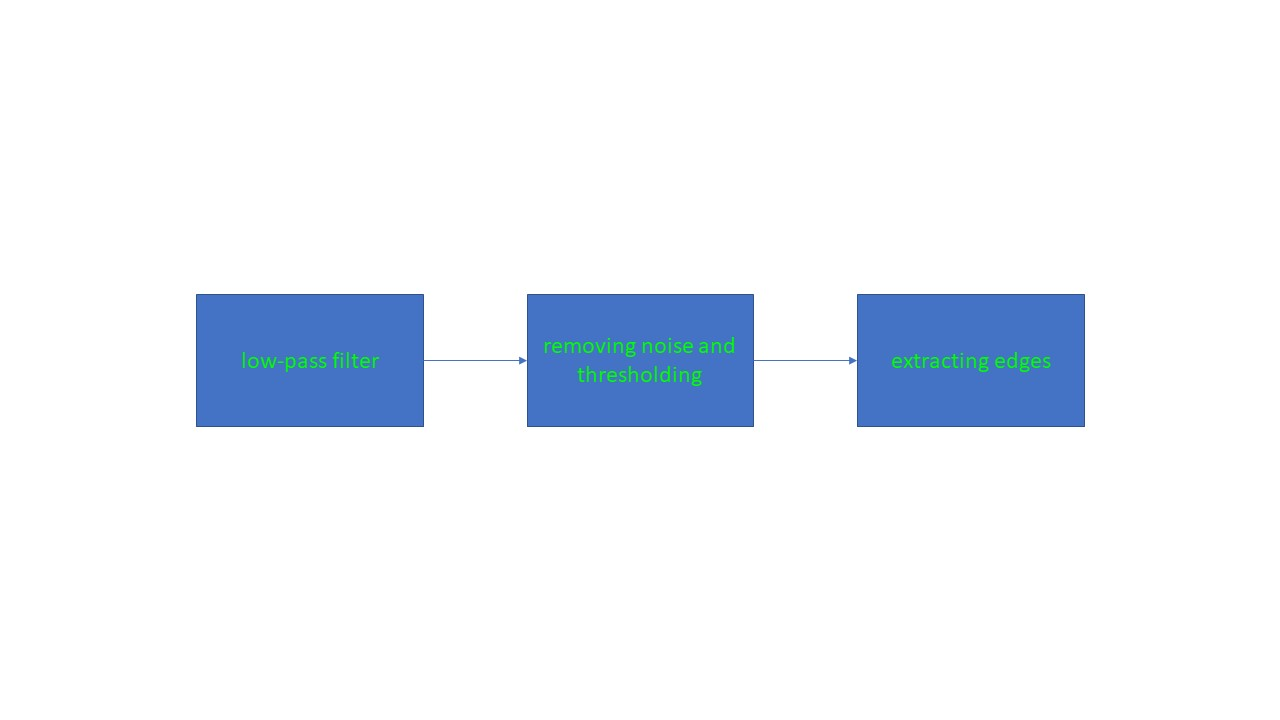
\includegraphics[width=1.0\textwidth]{figures/1.jpg}
%    \caption
%	{
%الگوهای مختلف در $LBP_{P,R}^{riu2}$
%	}
%    \label{fig:fig1}
%\end{figure}


\section{}%2
\subsection{فضای پیوسته}
شیب یک خط در فضای تصویر در بازه‌ی $\left( -\infty ,\: \infty \right)$ است. پس 
$
m \in \left( -\infty ,\: \infty \right)
$.
همچنین عرض از مبدا خط هم در فضای تصویر در بازه‌ی $\left( -\infty ,\: \infty \right)$ است. پس 
$
c \in \left( -\infty ,\: \infty \right)
$.
در نهایت فاصله‌ی خط از مبدا مختصات ($\rho$) در بازه‌ی $\left( 0 ,\: \sqrt{H^2 + W^2} \right)$ است که $H$ و $W$ به ترتیب عرض و طول تصویر هستند. پس 
$
\rho \in \left[ 0 ,\: \sqrt{H^2 + W^2} \right]
$.

\subsection{فضای گسسته}
با توجه به تصویر زیر و اینکه بیشینه‌ی مقدارِ $h$ برابر $H$ (که $H$ عرض تصویر است) پیکسل و کمینه‌ی مقدار $\epsilon$ برابر $1$ پیکسل است (وسط‌های پیکسل‌ها را در نظر می‌گیریم) شیب یک خط در فضای تصویر در بازه‌ی $\left[ -H ,\: H \right]$ است. البته شیب خط عمودی در تصویر تعریف نشده است. پس 
$
m \in \left[ -H ,\: H \right]
$.
\begin{figure}[H]
    \centering
    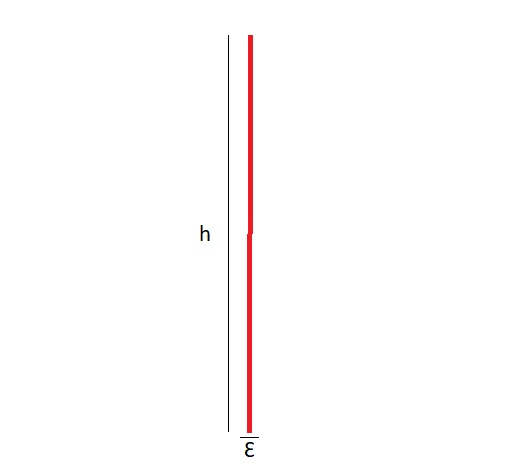
\includegraphics[width=0.5\textwidth]{figures/4.jpg}
    \caption
	{}
    \label{fig:fig1}
\end{figure}

همچنین عرض از مبدا خط هم در فضای تصویر در بازه‌ی $\left[ -\frac{H(W-2)}{2} ,\: \frac{H(W-2)}{2} \right]$ است. حالت بیشینه (کمینه) زمانی رخ می‌دهند که شیب بیشینه (کمینه) باشد. البته عرض از مبدا خط عمودی در تصویر تعریف نشده است. پس 
$
c \in \left[ -\frac{H(W-2)}{2} ,\: \frac{H(W-2)}{2} \right]
$.
در نهایت فاصله‌ی خط از مبدا مختصات ($\rho$) مثل حالت پیوسته در بازه‌ی $\left( 0 ,\: \sqrt{H^2 + W^2} \right)$ است که $H$ و $W$ به ترتیب عرض و طول تصویر هستند. پس 
$
\rho \in \left( 0 ,\: \sqrt{H^2 + W^2} \right)
$.


\section{}%3
هر دایره در فضای $x-y$ با 3 پارامتر مختصات مرکز و شعاع به صورت متمایز مشخص می‌شود. در نتیجه فضای هاف 3 بعدی است و هر نقطه در فضای هاف نظیر یک دایره در فضای $x-y$ است. همچنین دایره‌های نظیر هر دو نقطه‌ای که در فضای $x-y$ روی یک دایره قرار دارند، در فضای هاف از یک نقطه می‌گذرند که مختصات این نقطه (صرف نظر از مولفه‌ی نظیر شعاع) مختصات مرکز همان دایره در فضای $x-y$ است. معادله‌ی رویه‌ی مخروطی در فضای $x-y-z$، به شکل زیر است.
\newline
$$
\frac{(x-x_{0})^2}{a^2} + \frac{(y-y_{0})^2}{b^2} = \frac{(z-z_{0})^2}{c^2}
$$
با توجه به شباهت معادله‌ی دایره با سه پارامتر با معادله‌ی رویه‌ی مخروطی، نظیر همه‌ی دایره‌ها (شعاع‌های دلخواه)یی که در فضای $x-y$ از یک نقطه می‌گذرند یک رویه‌ی مخروطی در فضای هاف تشکیل می‌شود.
با استفاده از گسسته‌سازی فضا و مکانیزم انباشت‌گر (\lr{Accumulator}) به طریق الگوریتم زیر عمل می‌کنیم.

\begin{enumerate}
	\item تقسیم‌بندی فضای پارامترها یا $H$ به تعدادی سلول بر اساس دقت مورد انتظار با مقدار اولیه صفر
	\item به ازای هر نقطه (پیکسل سفید) با مختصات 
$(x_{i}, y_{i})$
 در صفحه تصویر
    \begin{enumerate}
		\item به ازای تمام مقادیر $r$ بین $r_{min}$ تا $r_{max}$
		\begin{enumerate}
			\item محاسبه‌ی مقدارِ
$H(x_{j}, y_{j}, r) = H(x_{j}, y_{j}, r) + 1$ به ازای تمام نقاط مثل $(x_{j}, y_{j})$ که روی دایره‌ی به مرکز $(x_{i}, y_{i})$ و شعاع $r$ قرار گرفته‌اند
		\end{enumerate}
    \end{enumerate}
    \item آنالیز داده‌ها در فضای هاف برای یافتن نقاط مطلوب (در واقع پیدا کردن مختصات نقطه‌ای که بیشترین $H$ را دارد)
    \item به دست آمدن مرکز دایره‌ی متناظر
\end{enumerate}


\section{}%4
\subsection{\lr{Algorithm}}
همانطور که در سوال قبل توضیح داده شد الگوریتم به شکل زیر است.
\begin{enumerate}
	\item تقسیم‌بندی فضای پارامترها یا $centers$ به تعدادی سلول بر اساس دقت مورد انتظار با مقدار اولیه صفر
	\item به ازای هر نقطه (پیکسل سفید) با مختصات 
$(i, j)$
 در صفحه تصویر
    \begin{enumerate}
		\item به ازای تمام مقادیر $r$ بین $40$ تا $50$
		\begin{enumerate}
			\item محاسبه‌ی مقدارِ
$centers(k, l, radius) = centers(k, l, radius) + 1$ به ازای تمام نقاط مثل $(k, l)$ که روی دایره‌ی به مرکز $(i, j)$ و شعاع $radius$ قرار گرفته‌اند
		\end{enumerate}
    \end{enumerate}
    \item آنالیز داده‌ها در فضای هاف برای یافتن نقاط مطلوب (در واقع پیدا کردن اندیس عنصر ماکسیمم آرایه‌ی $centers$)
    \item به دست آمدن مرکز/مراکز دایره‌/دایره‌های متناظر
\end{enumerate}
توجه شود که برای سادگی در پیاده‌سازی، تابع \lr{findCenters} در هر گام به ازای یک $radius$ خاص آرایه‌ی دو بعدی $centers$ را محاسبه می‌کند و سپس به آرایه‌ی 3 بعدی \lr{append} می‌شود.
\subsection{\lr{Function}}
\begin{latin}
\lstinputlisting{sources/findCenters.m}
\end{latin}

\subsection{\lr{Driver code}}
\begin{latin}
\lstinputlisting{sources/p4.m}
\end{latin}

\subsection{\lr{Block diagram}}
\begin{figure}[H]
    \centering
    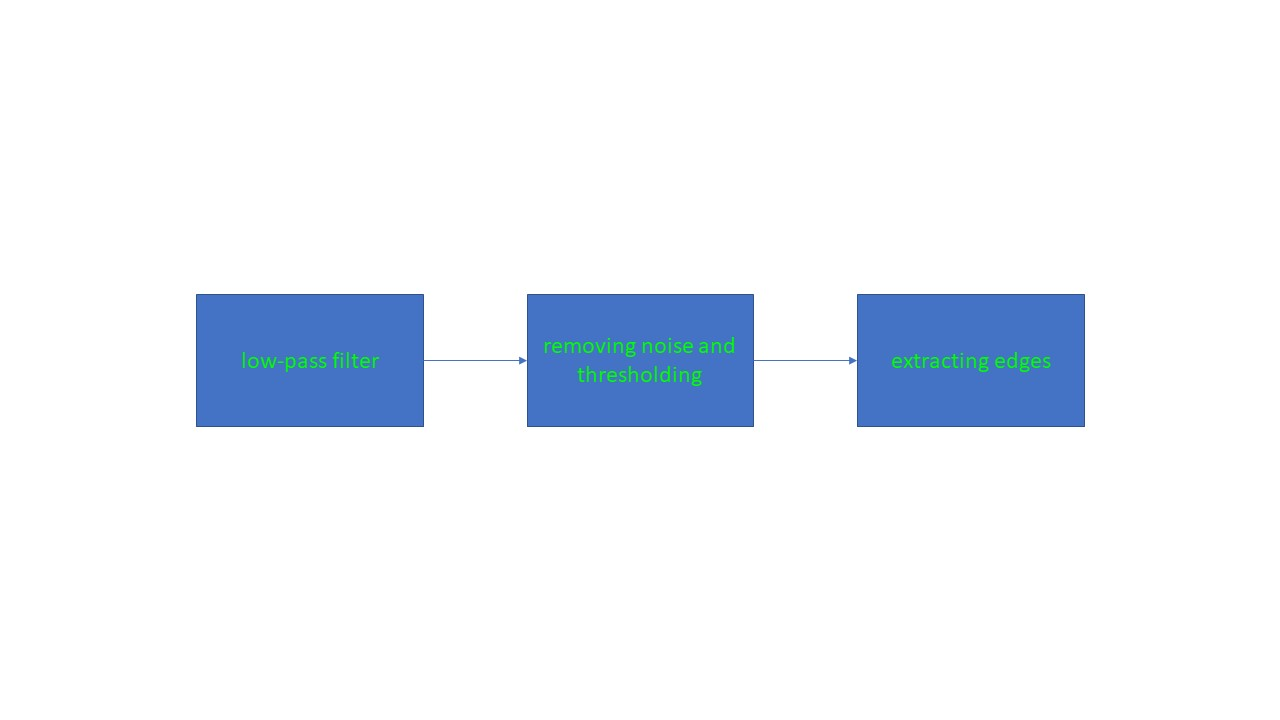
\includegraphics[width=1.0\textwidth]{figures/1.jpg}
    \caption
	{
بلوک‌دیاگرام پیش‌پردازش
	}
    \label{fig:fig1}
\end{figure}

\newpage
\subsection{\lr{Output}}
\begin{figure}[H]
    \centering
    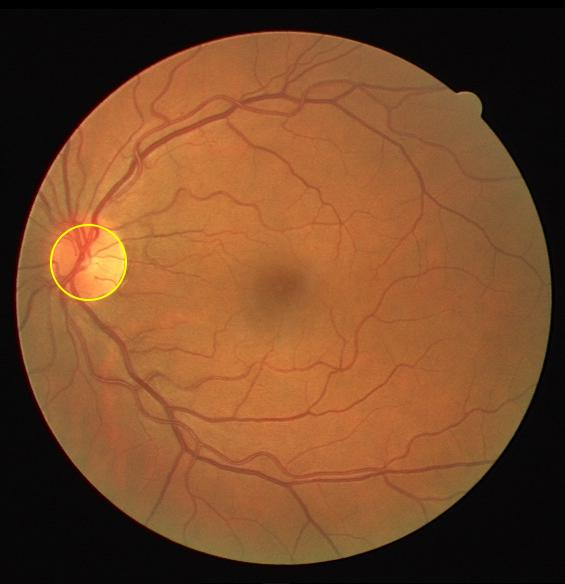
\includegraphics[width=0.5\textwidth]{figures/2.jpg}
    \caption
	{
مرکز دایره 
$(263, 89)$
است.
	}
    \label{fig:fig1}
\end{figure}
\begin{figure}[H]
    \centering
    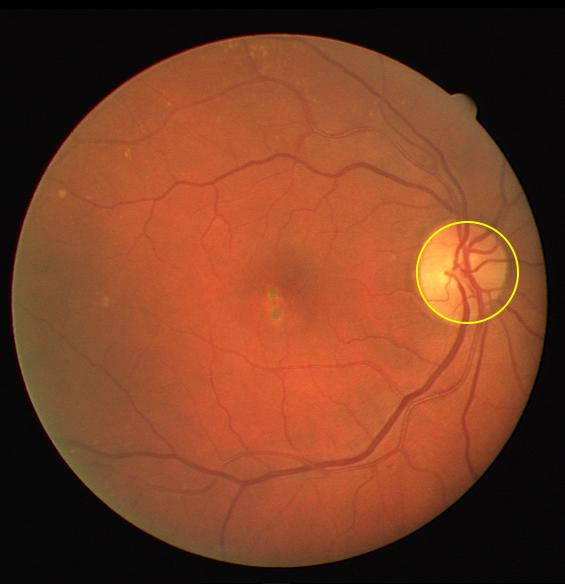
\includegraphics[width=0.5\textwidth]{figures/3.jpg}
    \caption
	{
مرکز دایره 
$(273, 468)$
است.
	}
    \label{fig:fig1}
\end{figure}



%%%%%%%%%%%%%%%%%%%%%%%%%%%%%%%%%%%
%%%%%%%%%%%%%%%%%%%%%%%%%%%%%%%%%%%
%%%%%%%%%%%%%%%%%%%%%%%%%%%%%%%%%%%

%------------------------------------------------------------------------------------------


\section*{منابع}
\renewcommand{\section}[2]{}%
\begin{thebibliography}{99} % assumes less than 100 references
%چنانچه مرجع فارسی نیز داشته باشید باید دستور فوق را فعال کنید و مراجع فارسی خود را بعد از این دستور وارد کنید


\begin{LTRitems}

\resetlatinfont

\bibitem{b1}
\end{LTRitems}

\end{thebibliography}


\end{document}
